\SourcePage{691}{696}
\section{Electron scattering by hadrons}

We apply the formulas obtained in the preceding section to elastic scattering of an electron by a hadron. Let $p_h$ and $p'_h$ denote the initial and final 4-momenta of the hadron, and let $p_e$ and $p'_e$ be those of the electron; then
\begin{equation}
p_e+p_h=p'_e+p'_h.
\tag{139.1}
\end{equation}
The process under consideration is represented by the diagram
\begin{equation}
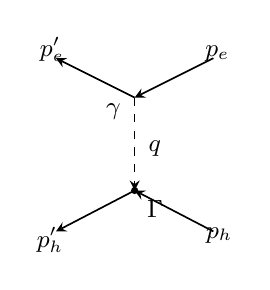
\begin{tikzpicture}[baseline=-.45ex,x=1cm,y=1cm,>=stealth,line width=.6pt,font=\small]
  \coordinate (ve) at (0,.70);
  \coordinate (vh) at (0,-.48);
  \draw[->] (1.00,1.20)--(ve);
  \draw[->] (ve)--(-1.00,1.20);
  \draw[dashed,->] (ve)--(vh);
  \draw[->] (1.00,-1.00)--(vh);
  \draw[->] (vh)--(-1.00,-1.00);
  \fill (vh) circle (1.3pt);
  \node[above right] at (.77,1.03) {$p_e$};
  \node[above left] at (-.77,1.03) {$p'_e$};
  \node[below right] at (.78,-.82) {$p_h$};
  \node[below left] at (-.78,-.82) {$p'_h$};
  \node[left] at (-.05,.52) {$\gamma$};
  \node[right] at (.05,.05) {$q$};
  \node[below right] at (.03,-.48) {$\Gamma$};
\end{tikzpicture}
\tag{139.2}
\end{equation}
Emission of the virtual photon by the electron is described by the usual vertex operator $\gamma$, while its absorption by the hadron is described by the operator $\Gamma$.

Consider the most interesting case, a hadron of spin $1/2$ (for example, electron scattering by a proton or neutron). The scattering amplitude associated with diagram~(139.2) is
\begin{equation}
M_{fi}=-4\pi e^2\frac{1}{q^2}(\bar u'_e\gamma^\mu u_e)(\bar u'_h\Gamma_\mu u_h)
\tag{139.3}
\end{equation}
(throughout this chapter the electron charge is $-e$!). Computing the cross section from this amplitude involves no difference of principle from the calculations in~\S~81; for this purpose it is convenient to write the operator $\Gamma$ in the first of the forms~(138.7).

\SourcePage{692}{697}
For unpolarized particles the result is
\begin{equation}
\begin{aligned}
d\sigma={}&\frac{\pi\alpha^2\,dt}
{[s-(M+m)^2][s-(M-m)^2]t^2(1-t/4M^2)}\times{}\\
&\times\left\{F_e^2\bigl[(s-u)^2+(4M^2-t)t\bigr]
-\frac{t}{4M^2}F_m^2\bigl[(s-u)^2-(4M^2-t)(4m^2+t)\bigr]\right\}.
\end{aligned}
\tag{139.4}
\end{equation}
Here $M$ is the hadron mass, $m$ is the electron mass, and
\[
s=(p_e+p_h)^2,\qquad t=q^2=(p_e-p'_e)^2,\qquad u=(p_e-p'_h)^2,
\]
\[
s+t+u=2m^2+2M^2.
\]

We shall examine several limiting cases.

For electrons scattered by a heavy nucleus, the case of interest is one in which the momentum $|\mathbf q|$ transferred from the electron to the nucleus is small relative to the nuclear mass, but not relative to $1/R$ (where $R$ is the nuclear radius), so that the nucleus cannot be regarded as pointlike. The centre-of-mass system then approximately coincides with the rest frame of the nucleus, its recoil may be neglected, and the electron energy remains unchanged. Thus
\[
-t=\mathbf q^2\ll M^2,\qquad \pi|dt|=\mathbf p_e^2do'_e,\qquad s-M^2\approx M^2-u\approx2M\varepsilon_e
\]
and formula~(139.4) becomes
\begin{equation}
d\sigma=\frac{\alpha^2do'_e}{\mathbf q^4}(4\varepsilon_e^2-\mathbf q^2)F_e^2(-\mathbf q^2).
\tag{139.5}
\end{equation}
In this approximation, only the term containing the electric form factor remains in the cross section, and~(139.5) agrees with formula~(80.5) for electron scattering by a static charge distribution.

For an electron scattered by a neutron at rest in the same limiting case $\varepsilon_e\ll M$ (where $M$ is the neutron mass), the form factors may be replaced by their values at $\mathbf q=0$. Indeed, as noted already, the characteristic ``radius'' of the charge distribution of a single nucleon is comparable with $1/M$\footnote{The empirical root-mean-square nucleon ``radius'' is $\approx3{,}5/M\approx1/(2m_\pi)$ (where $m_\pi$ is the pion mass).}. Since the neutron is electrically neutral, $F_e(0)=0$, and the cross section takes the form
\begin{equation}
d\sigma=\alpha\mu^2\left[\frac{4(\varepsilon_e^2-m^2)}{\mathbf q^2}+1\right]do'_e
=\alpha\mu^2\left(\frac{1}{\sin^2(\vartheta/2)}+1\right)do'_e,
\tag{139.6}
\end{equation}
where $\mu=\dfrac{e}{2M}F_m(0)$ is the neutron magnetic moment and $\vartheta$ is the scattering angle. This formula describes scattering of an electron by a stationary point magnetic moment.

\SourcePage{693}{698}
Finally, let us give the cross section for an ultrarelativistic electron scattered by a nucleon when $|\mathbf q|\gg m$. As before, $\mathbf q^2$ denotes the square of the momentum transfer in the centre-of-mass system, so that the invariant is $t=-\mathbf q^2$. In the rest frame of the initial nucleon (the laboratory frame), however,
\[
-t\approx2(p_ep'_e)=2\varepsilon_e\varepsilon'_e(1-\cos\vartheta),
\]
where $\varepsilon_e$ and $\varepsilon'_e$ are the initial and final electron energies, while $\vartheta$ is the scattering angle in this frame. In the ultrarelativistic case, $\varepsilon'_e$ is related to $\vartheta$ by the same formula as in photon scattering (cf.~(86.8)):
\[
\frac{1}{\varepsilon'_e}-\frac{1}{\varepsilon_e}=\frac{1}{M}(1-\cos\vartheta).
\]
Consequently,
\begin{equation}
-t=\frac{4\varepsilon_e^2\sin^2(\vartheta/2)}
{1+\dfrac{2\varepsilon_e}{M}\sin^2(\vartheta/2)},
\tag{139.7}
\end{equation}
\begin{equation}
\pi d|t|=\frac{\varepsilon_e^2do'_e}
{\left(1+\dfrac{2\varepsilon_e}{M}\sin^2(\vartheta/2)\right)^2},
\tag{139.8}
\end{equation}
where $do'_e=2\pi\sin\vartheta\,d\vartheta$. The electron mass $m$ may be omitted throughout formula~(139.4); expressing all quantities in terms of $t$ and $s-M^2=2M\varepsilon_e$, we obtain
\begin{equation}
\begin{aligned}
d\sigma={}&\frac{\pi\alpha^2d|t|}{\varepsilon_e^2t^2}
\left\{F_e^2(t)\left[\frac{(4M\varepsilon_e+t)^2}{4M^2-t}+t\right]\right.\\
&\left.\hspace{6em}{}-\frac{t}{4M^2}F_m^2(t)
\left[\frac{(4M\varepsilon_e+t)^2}{4M^2-t}-t\right]\right\},
\end{aligned}
\tag{139.9}
\end{equation}
or, on using~(139.7), (139.8),
\begin{equation}
\begin{aligned}
d\sigma={}&do'_e\frac{\alpha^2}{4\varepsilon_e^2}
\frac{\cos^2(\vartheta/2)}{\sin^4(\vartheta/2)}
\frac{1}{1+\dfrac{2\varepsilon_e}{M}\sin^2(\vartheta/2)}\times{}\\
&\times\left\{\frac{F_e^2-\dfrac{t}{4M^2}F_m^2}{1-\dfrac{t}{4M^2}}
-\frac{t}{2M^2}F_m^2\tan^2\frac{\vartheta}{2}\right\}.
\end{aligned}
\tag{139.10}
\end{equation}
(\emph{M.~Rosenbluth}, 1950).

Notice that $F_e$ and $F_m$ contribute independently to the cross section: there are no interference terms. This confirms the usefulness of the chosen form factors.

\ProblemHeading

Find the cross section for electron scattering by a spin-zero hadron.

\SolutionHeading Using~(138.5), in place of~(139.3) we have
\[
M_{fi}=-\frac{4\pi e^2}{q^2}\bigl(\bar u'_e(\gamma P)u_e\bigr)F(q^2).
\]

\SourcePage{694}{699}
The cross section is therefore
\[
d\sigma=\frac{\pi\alpha^2dt\bigl[(s-u)^2+(4M^2-t)t\bigr]}
{[s-(M+m)^2][s-(M-m)^2]t^2}F^2(t)
\]
(the notation is the same as in~(139.4)). For $|t|\gg m^2$,
\[
d\sigma=do'_e\frac{\alpha^2}{4\varepsilon_e^2}
\frac{\cos^2(\vartheta/2)}{\sin^4(\vartheta/2)}
\frac{F^2(t)}{1+\dfrac{2\varepsilon_e}{M}\sin^2(\vartheta/2)}
\]
(the notation is the same as in~(139.10)).
